\chapter{Conception du système}

\section{Architecture générale}

L'application adopte une \textbf{architecture en couches}, qui consiste à séparer le code en couches successives, chacune ayant une responsabilité bien définie. Cette organisation favorise la lisibilité, la maintenabilité et la réutilisation du code.

La figure~\ref{fig:architecture} illustre l'empilement des couches de l'application, du haut vers le bas :

\begin{itemize}
    \item la couche \textbf{présentation}, constituée de pages JSP enrichies par la bibliothèque JSTL, est responsable de l'affichage des données et de la saisie par l'utilisateur ;
    \item la couche \textbf{contrôleur}, composée de servlets, reçoit les requêtes HTTP, délègue le traitement à la couche métier et sélectionne la vue à afficher ;
    \item la couche \textbf{métier} (service) implémente la logique applicative et applique les règles de gestion ;
    \item la couche d'\textbf{accès aux données} (DAO), fondée sur JPA/Hibernate, assure la persistance des entités et l'exécution des requêtes ;
    \item la base de données \textbf{MySQL} stocke physiquement les informations.
\end{itemize}

\begin{figure}[H]
\centering
\begin{tikzpicture}[
    node distance=0.65cm,
    layer/.style={draw, rounded corners=2pt, minimum width=10cm, minimum height=0.9cm, align=center, font=\small},
    arrow/.style={-{Stealth}, thick}
]
\node[layer] (vue) {Couche Présentation\\ (JSP + JSTL)};
\node[layer, below=of vue] (ctrl) {Couche Contrôleur\\ (Servlets)};
\node[layer, below=of ctrl] (svc) {Couche Métier\\ (Services)};
\node[layer, below=of svc] (dao) {Couche d'Accès aux Données\\ (DAO + JPA/Hibernate)};
\node[layer, below=of dao] (db) {Base de Données\\ (MySQL)};

\draw[arrow] (vue) -- (ctrl);
\draw[arrow] (ctrl) -- (svc);
\draw[arrow] (svc) -- (dao);
\draw[arrow] (dao) -- (db);
\end{tikzpicture}
\caption{Architecture en couches de l'application}
\label{fig:architecture}
\end{figure}

Le flux d'une requête est le suivant : la servlet reçoit la requête, appelle le service concerné, qui fait appel à la couche DAO pour lire ou écrire en base de données, puis la servlet transmet les résultats à la JSP chargée de les afficher.

\section{Diagramme de classes}

Le diagramme de classes (figure~\ref{fig:classes}) décrit la structure statique du système : les entités, leurs attributs et les relations qui les unissent. Il constitue la base de la modélisation objet et de la persistance JPA.

\begin{figure}[H]
\centering
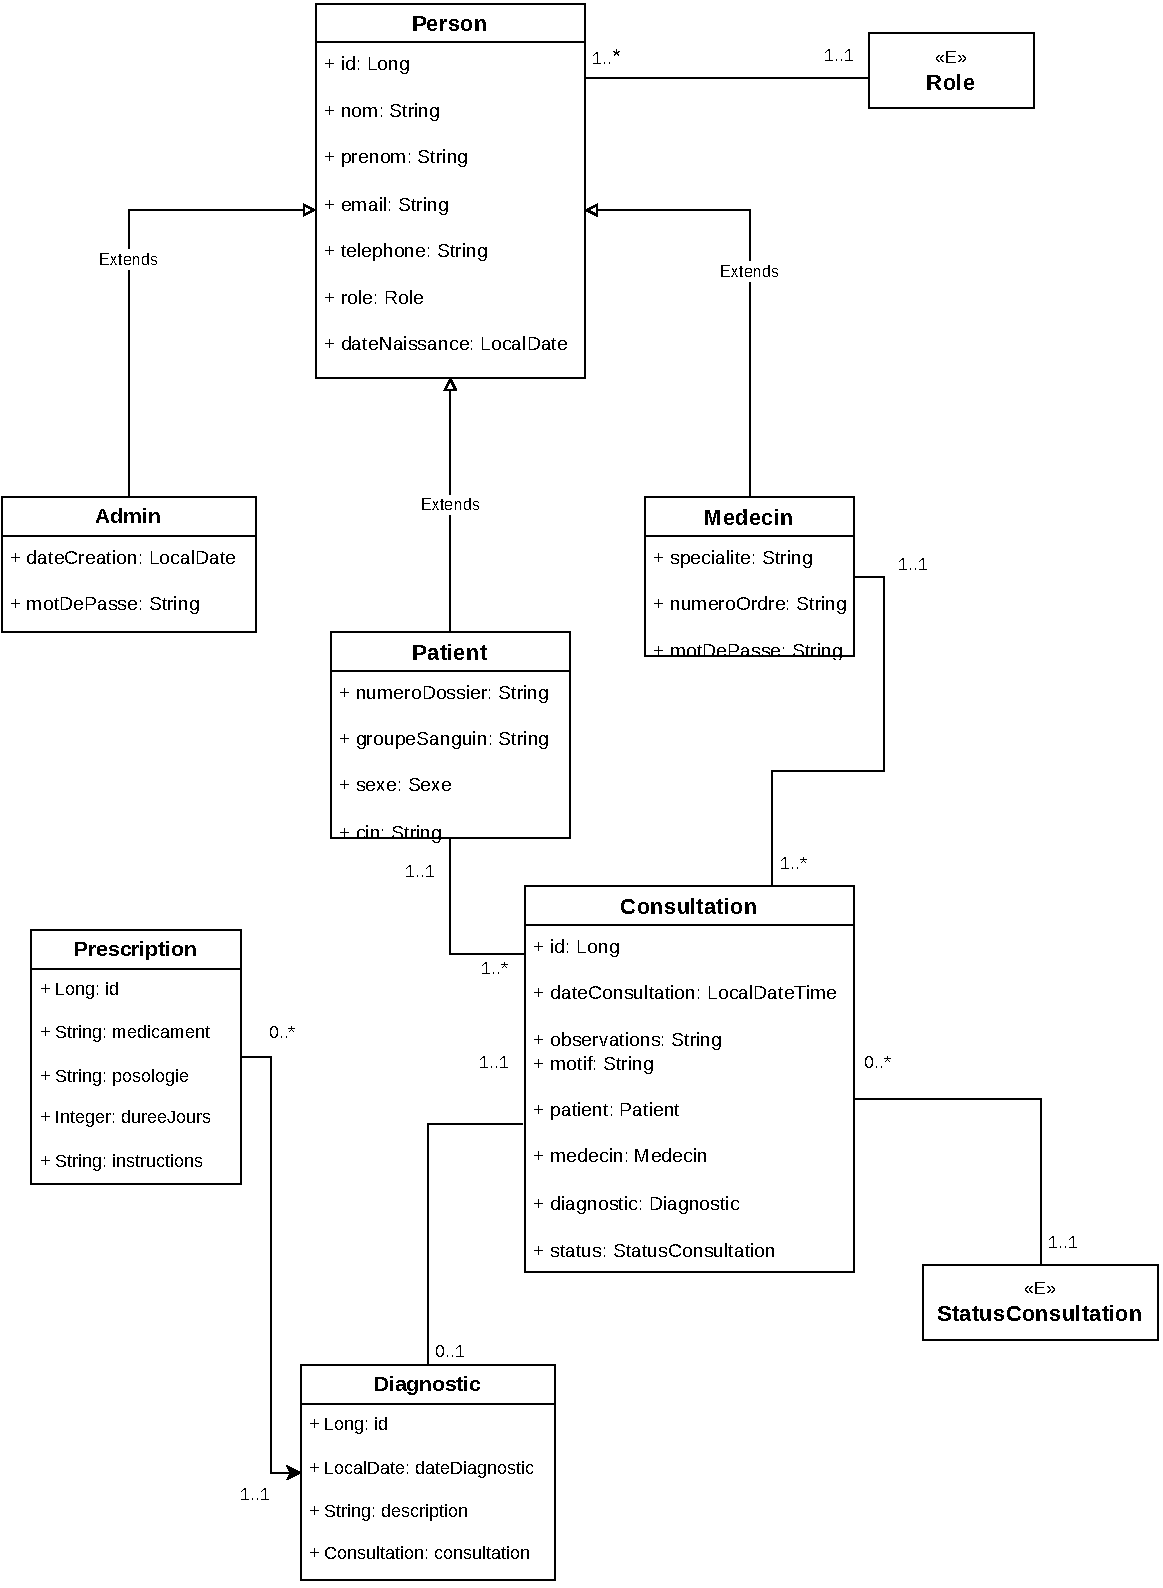
\includegraphics[width=\textwidth]{images/diagramme-classes}
\caption{Diagramme de classes du système}
\label{fig:classes}
\end{figure}

\subsection{Les entités}

La classe abstraite \textbf{Person} regroupe les attributs communs à tous les utilisateurs : identifiant, nom, prénom, email, téléphone, date de naissance et rôle. Elle est annotée \texttt{@MappedSuperclass} dans le code, ce qui signifie que ses colonnes sont héritées dans la table de chacune de ses sous-classes. Trois entités en héritent :

\begin{itemize}
    \item \textbf{Patient}, qui ajoute le numéro de dossier, le groupe sanguin, le sexe, le CIN et l'adresse ;
    \item \textbf{Medecin}, qui ajoute la spécialité, le numéro d'ordre et le mot de passe ;
    \item \textbf{Admin}, qui ajoute le mot de passe et la date de création du compte.
\end{itemize}

Les entités \textbf{Consultation}, \textbf{Diagnostic} et \textbf{Prescription} modélisent le cœur métier. Une consultation associe un patient et un médecin à une date donnée, possède un motif, des observations et un statut. Elle peut donner lieu à un diagnostic, lequel peut contenir une ou plusieurs prescriptions.

\subsection{Les relations}

Les relations entre les entités, assorties de leurs multiplicités, sont les suivantes :

\begin{itemize}
    \item un \textbf{Patient} possède une ou plusieurs \textbf{Consultation}s (1..*), et chaque consultation appartient à un seul patient (1..1) ;
    \item un \textbf{Medecin} possède une ou plusieurs \textbf{Consultation}s (1..*), et chaque consultation est assurée par un seul médecin (1..1) ;
    \item une \textbf{Consultation} peut avoir au plus un \textbf{Diagnostic} (0..1), et chaque diagnostic est lié à une seule consultation (1..1) ;
    \item un \textbf{Diagnostic} peut contenir plusieurs \textbf{Prescription}s (0..*), et chaque prescription est rattachée à un seul diagnostic (1..1) ;
    \item chaque \textbf{Person} possède un seul \textbf{Role} (1..1), et un même rôle est partagé par plusieurs personnes (1..*).
\end{itemize}

\subsection{Les énumérations}

Trois énumérations structurent le modèle :

\begin{itemize}
    \item \textbf{Role} : ADMIN, MEDECIN, PATIENT ;
    \item \textbf{Sexe} : HOMME, FEMME ;
    \item \textbf{StatusConsultation} : Planifiée, Terminée, Annulée.
\end{itemize}

\section{Diagramme d'états-transitions}

Le diagramme d'états-transitions (figure~\ref{fig:etats}) décrit le \textbf{cycle de vie d'une consultation}, c'est-à-dire les différents états qu'elle peut prendre et les événements qui provoquent le passage d'un état à un autre.

\begin{figure}[H]
\centering
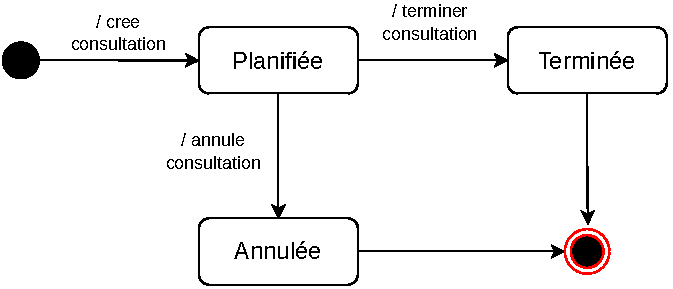
\includegraphics[width=0.85\textwidth]{images/diagramme-etats}
\caption{Diagramme d'états-transitions d'une consultation}
\label{fig:etats}
\end{figure}

Le cycle de vie est le suivant :

\begin{itemize}
    \item à sa création, la consultation entre dans l'état \textbf{Planifiée} ;
    \item depuis l'état \textbf{Planifiée}, la consultation peut passer à l'état \textbf{Terminée} lorsque le médecin la clôture, ou à l'état \textbf{Annulée} lorsque l'administrateur l'annule ;
    \item les états \textbf{Terminée} et \textbf{Annulée} constituent les états finaux du cycle de vie.
\end{itemize}

Ce cycle correspond directement à l'énumération \texttt{StatusConsultation} du modèle : la valeur par défaut d'une nouvelle consultation est « Planifiée », puis elle évolue vers « Terminée » ou « Annulée ».

\section{Dictionnaire de données}

Le \textbf{dictionnaire de données} est un document de référence qui recense, de manière exhaustive, l'ensemble des données manipulées par le système. Pour chaque donnée, il précise son nom, son type, sa taille, ses contraintes (obligatoire, unique, clé étrangère\ldots) et sa signification.

Son intérêt est double. D'une part, il constitue un \textbf{référentiel commun} entre les différents intervenants du projet, garantissant que chaque donnée est désignée et comprise de la même manière par tous. D'autre part, il sert de \textbf{base à la conception de la base de données} : chaque entité du modèle objet correspond à une table, et chaque attribut à une colonne dont le type et les contraintes découlent directement du dictionnaire.

Le tableau~\ref{tab:dictionnaire} présente le dictionnaire de données du système, organisé par entité.

\begin{center}
\small
\begin{longtable}{p{2.7cm} p{2.6cm} p{1.5cm} p{3.4cm} p{5.2cm}}
\caption{Dictionnaire de données du système}
\label{tab:dictionnaire} \\
\toprule
\textbf{Attribut} & \textbf{Type} & \textbf{Taille} & \textbf{Contraintes} & \textbf{Description} \\
\midrule
\endfirsthead
\toprule
\textbf{Attribut} & \textbf{Type} & \textbf{Taille} & \textbf{Contraintes} & \textbf{Description} \\
\midrule
\endhead
\bottomrule
\endlastfoot

\multicolumn{5}{l}{\textbf{Person (classe de base)}} \\
id & Long & -- & Clé primaire, auto-incrément & Identifiant unique \\
nom & String & 50 & Non nul & Nom \\
prenom & String & 50 & Non nul & Prénom \\
email & String & 100 & Non nul, unique & Adresse email (identifiant de connexion) \\
telephone & String & 20 & -- & Numéro de téléphone \\
role & Role (enum) & 30 & Non nul & Rôle : ADMIN, MEDECIN, PATIENT \\
dateNaissance & LocalDate & -- & -- & Date de naissance \\
\midrule

\multicolumn{5}{l}{\textbf{Patient (hérite de Person)}} \\
numeroDossier & String & 20 & Unique & Numéro de dossier médical \\
groupeSanguin & String & 5 & -- & Groupe sanguin \\
sexe & Sexe (enum) & 10 & Non nul & Sexe : HOMME, FEMME \\
cin & String & 20 & Non nul, unique & Carte d'identité nationale \\
adresse & String & 255 & -- & Adresse \\
\midrule

\multicolumn{5}{l}{\textbf{Medecin (hérite de Person)}} \\
specialite & String & 80 & -- & Spécialité médicale \\
numeroOrdre & String & 20 & Unique & Numéro d'ordre des médecins \\
motDePasse & String & -- & Non nul & Mot de passe de connexion \\
\midrule

\multicolumn{5}{l}{\textbf{Admin (hérite de Person)}} \\
motDePasse & String & -- & Non nul & Mot de passe de connexion \\
dateCreation & LocalDate & -- & -- & Date de création du compte \\
\midrule

\multicolumn{5}{l}{\textbf{Consultation}} \\
id & Long & -- & Clé primaire, auto-incrément & Identifiant unique \\
dateConsultation & LocalDateTime & -- & Non nul & Date et heure de la consultation \\
observations & String & 2000 & -- & Observations du médecin \\
motif & String & 255 & -- & Motif de la consultation \\
patient & Patient & -- & Non nul, clé étrangère & Patient concerné \\
medecin & Medecin & -- & Non nul, clé étrangère & Médecin assurant la consultation \\
diagnostic & Diagnostic & -- & -- & Diagnostic associé \\
status & StatusConsultation (enum) & 30 & Non nul, défaut « Planifiée » & Statut de la consultation \\
\midrule

\multicolumn{5}{l}{\textbf{Diagnostic}} \\
id & Long & -- & Clé primaire, auto-incrément & Identifiant unique \\
dateDiagnostic & LocalDate & -- & -- & Date du diagnostic \\
description & String & 1000 & Non nul & Description du diagnostic \\
consultation & Consultation & -- & Non nul, unique, clé étrangère & Consultation associée \\
prescriptions & Liste de Prescription & -- & -- & Prescriptions associées \\
\midrule

\multicolumn{5}{l}{\textbf{Prescription}} \\
id & Long & -- & Clé primaire, auto-incrément & Identifiant unique \\
medicament & String & 100 & Non nul & Nom du médicament \\
posologie & String & 100 & Non nul & Posologie (dosage) \\
dureeJours & Integer & -- & -- & Durée du traitement en jours \\
instructions & String & 300 & -- & Instructions complémentaires \\
diagnostic & Diagnostic & -- & Non nul, clé étrangère & Diagnostic associé \\
\bottomrule
\end{longtable}
\end{center}

Le tableau~\ref{tab:enums} récapitule les valeurs des différentes énumérations utilisées dans le modèle.

\begin{table}[H]
\centering
\begin{tabularx}{\textwidth}{l l X}
\toprule
\textbf{Énumération} & \textbf{Valeurs} & \textbf{Signification} \\
\midrule
Role & ADMIN, MEDECIN, PATIENT & Rôle d'un utilisateur du système \\
Sexe & HOMME, FEMME & Sexe d'un patient \\
StatusConsultation & Planifiée, Terminée, Annulée & Cycle de vie d'une consultation \\
\bottomrule
\end{tabularx}
\caption{Valeurs des énumérations du modèle}
\label{tab:enums}
\end{table}
